\begin{figure}[htbp]{fig:4-primer_grafo}{Grafo obtenido del artículo~\cite{multi-objective_routing_optimization}}
  \centering
  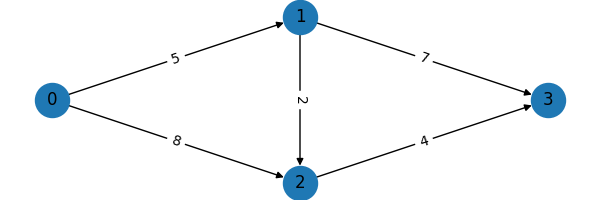
\includegraphics[scale=0.75]{primer-grafo/primer-grafo}
\end{figure}

En la \textit{sección~\ref{sec:4-tutorial_de_qiskit}} se consiguieron replicar los cálculos teóricos de una instancia de QAOA simple, sin restricciones y poco profunda. Por ello el siguiente problema a resolver aumenta su complejidad, añadiendo restricciones y aumentando la cantidad de qubits del sistema. \\
En esta sección se pretenden imitar los resultados obtenidos en la sección 2.2 (\textit{Single-Objective Quantum Routing Optimization}) del \textit{artículo~\cite{multi-objective_routing_optimization}}.

El problema consiste en encontrar el camino más corto que conecte los nodos \textit{0} y \textit{3}.
\begin{itemize}
\item \textbf{Objetivo:}

  \begin{align*}
    &\min(5X_{01} + 8X_{02} + 2X_{12} + 7X_{13} + 4X_{23}) \\
    &\textnormal{dde } X_{ij} = \begin{cases}
      1 \textnormal{ si el camino contiene la arista del nodo \textit{i} al \textit{j}} \\
      0 \textnormal{ en otro caso}
    \end{cases}
  \end{align*}
  
\item \textbf{Restricciones:}
  También se deben añadir una serie de restricciones para evitar caminos triviales o incongruentes.

  \begin{enumerate}
  \item\label{it:4-primer_grafo_restriccion_ini} $X_{01} + X_{02} = 1$:
    Debe haber exactamente un eje del camino que involucre al nodo de comienzo.
    Obliga al camino a comenzar por dicho nodo.

  \item\label{it:4-primer_grafo_restriccion_inter} $X_{01} = X_{12} + X_{13} \\
    X_{02} + X_{12} = X_{23}$:
    Para cada nodo intermedio debe haber en el resultado tantas aristas entrantes como salientes.
    Evita caminos incongruentes y hace que el único nodo posible para finalizar sea el nodo final.
  \end{enumerate}

  Siguiendo el caso del artículo se elige como valor del \textit{modificador de Lagrange} \(P=27\), ya que debe ser estrictamente mayor que el máximo de la función objetivo:
  \(\max_{x}{f_{\textnormal{sin restricc}}(x)} = \sum_{(i, j)\in{E}}{w_{ij}} = 26\)

\end{itemize}

De acuerdo con los pasos descritos en la \textit{sección~\ref{sec:3-problemas de optimizacion combinatoria}}, la función de coste clásica en su versión QUBO es:

\begin{align*}
  f(X) &= 5X_{01} + 8X_{02} + 2X_{12} + 7X_{13} + 4X_{23} + \\
       &+ P{(X_{01} + X_{02} - 1)}^2 + P{(X_{01} - X_{12} - X_{13})}^2 + P{(X_{02} + X_{12} - X_{23})}^2
\end{align*}

El número de qubits del sistema cuántico es igual a la cantidad de variables de la función de coste, esto es, la cantidad de ejes del grafo. \\
Las variables X de la función de coste tienen valores 0 o 1 y para la conversión a su correspondiente función de coste implementada en un circuito cuántico se utiliza la formulación Ising.  % TODO: Citar Ising formulation for many np problems????
Estas nuevas variables ($z$) van a tomar valores -1 y 1 y cada variable $z_k$ estará asociada al qubit k-ésimo del circuito. En este caso la correspondencia entre $X_{ij}$ y $z_k$ es la siguiente:
$X_{01}$ corresponde con $z_0$,
$X_{02}$ corresponde con $z_1$,
$X_{12}$ corresponde con $z_2$,
$X_{13}$ corresponde con $z_3$ y
$X_{23}$ corresponde con $z_4$.

Como ya se ha visto en la sección  % TODO: Citar sección correspondiente de Diseño
cada variable $z_i$ va a corresponder con una puerta Pauli-Z en el qubit i.

De acuerdo con la \textit{sección~\ref{sec:3-operador c}} la versión Ising de la función de coste queda como:

\begin{align*}
  g(z) = &5\frac{1-z_0}{2} + 8\frac{1-z_1}{2} + 2\frac{1-z_2}{2} + 7\frac{1-z_3}{2} + 4\frac{1-z_4}{2} + \\
         &+ P{(\frac{1-z_0}{2} + \frac{1-z_1}{2} - 1)}^2 + P{(\frac{1-z_0}{2} - \frac{1-z_2}{2} - \frac{1-z_3}{2})}^2 + \\
         &+ P{(\frac{1-z_1}{2} + \frac{1-z_2}{2} - \frac{1-z_4}{2})}^2 = \\
  = & 11z_0 - 17.5z_1 - 28z_2 - 17z_3 + 11.5z_4 + \\
         &+ 13.5(z_0z_1 - z_0z_2 - z_0z_3 + z_1z_2 - z_1z_4 + z_2z_3 - z_2z_4) + \\
         &+ 80.5 \\
\end{align*}
\par
Esta igualdad solo se cumple para variables con valores \(\{-1, 1\}\), ya que \(z_i^2 = 1\). \\

\par
De forma similar a la \textit{sección~\ref{sec:4-tutorial_de_qiskit}} se obtiene el hamiltoniano $U(C, \gamma)$ a partir de $g(z)$:

\begin{align*}
  &U(C, \gamma) = \exp(-i \gamma C) = \\
  &= Rz_0(11*2\gamma) \cdot Rz_1(-17.5*2\gamma) \cdot Rz_2(-28*2\gamma) \cdot Rz_3(-17*2\gamma) \cdot Rz_4(11.5*2\gamma) \cdot \\
  & \cdot Rz_0z_1(+13.5 * 2\gamma) \cdot Rz_0z_2(-13.5 * 2\gamma) \cdot Rz_0z_3(-13.5 * 2\gamma) \cdot Rz_1z_2(+13.5 * 2\gamma) \cdot \\
  & \cdot Rz_1z_4(-13.5 * 2\gamma) \cdot Rz_2z_3(+13.5 * 2\gamma) \cdot Rz_2z_4(-13.5 * 2\gamma)
\end{align*}

Con el operador \(U(B, \beta)\) y el vector inicial, definidos en la \textit{sección~\ref{sec:3-circuito de qaoa}}, y el operador \(U(C, \gamma)\) obtenido se puede construir el circuito cuántico.

\begin{figure}[htbp]{}{ Circuito obtenido ($p=1$) }
  \centering
  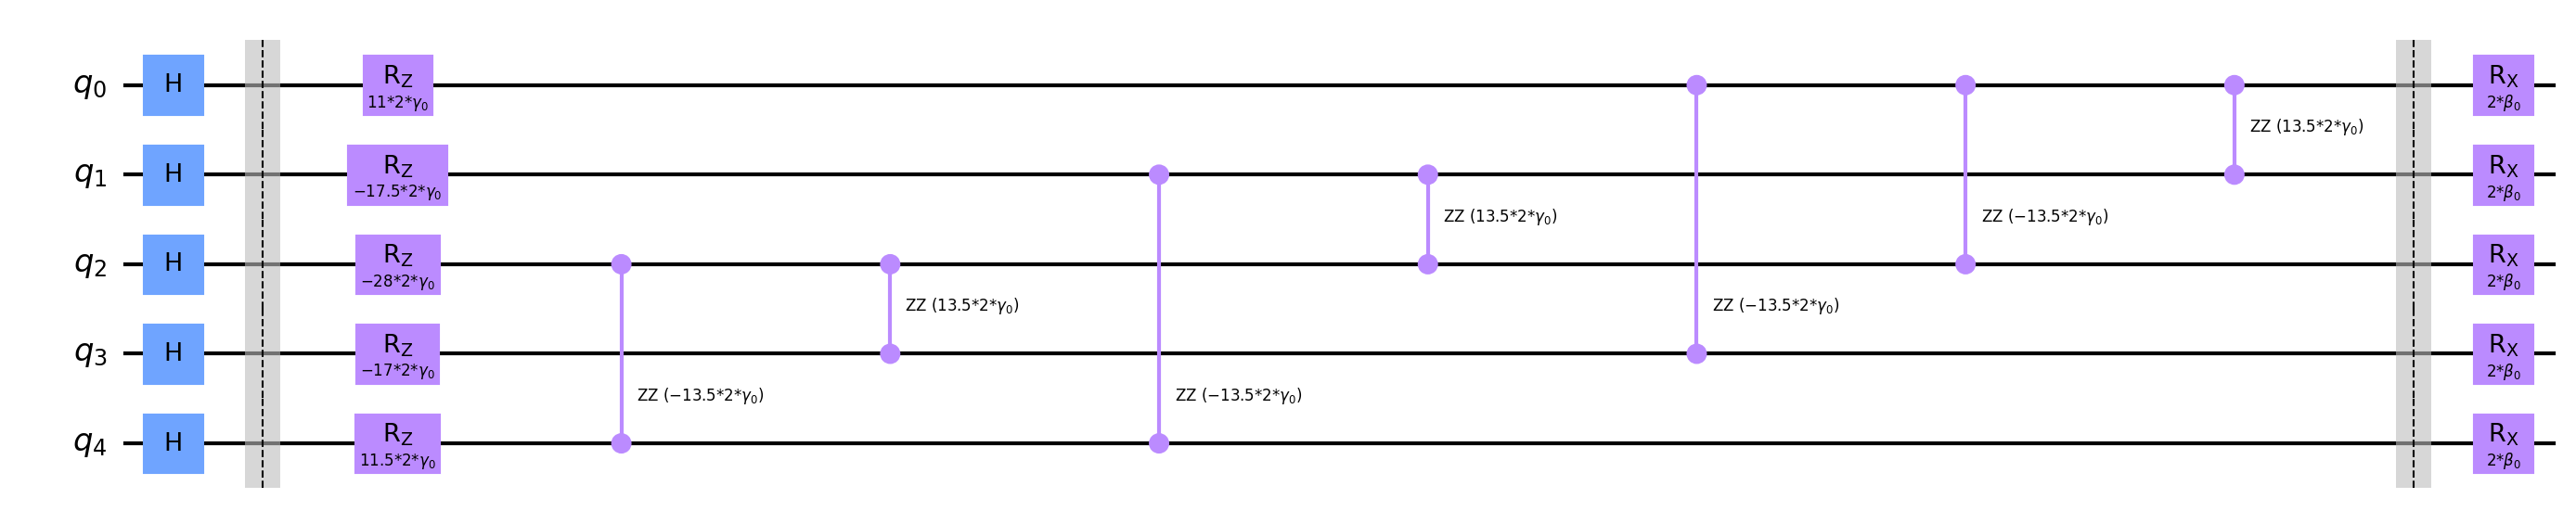
\includegraphics[scale=0.27]{circuits/primer/primer-circuit-2gamma-p1.png}
\end{figure}

\begin{figure}[htbp]{fig:4-primer_paper_circuito}{ Circuito del artículo ($p=1$) }
  \centering
  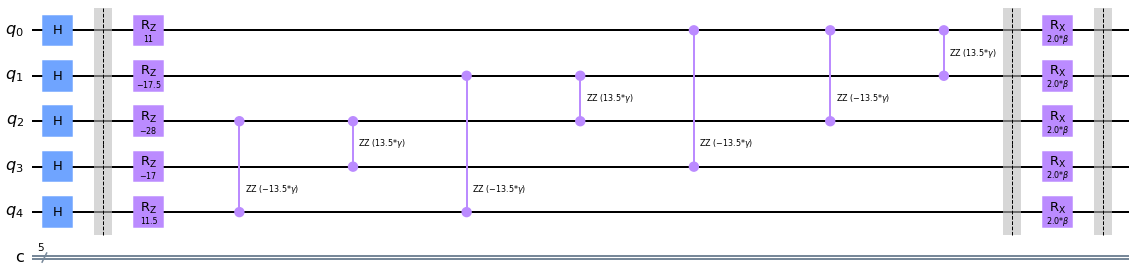
\includegraphics[scale=0.3]{circuits/paper/paper-circuit.png}
\end{figure}

\paragraph{Diferencias con el artículo\label{sec:4-primer_grafo_diferencias_con_el_articulo}}
El \textit{circuito~\ref{fig:4-primer_paper_circuito}} obtenido teóricamente difiere del que se puede ver en la sección 2.2 del \textit{artículo~\cite{multi-objective_routing_optimization}}. \\
En la sección anterior se obtienen operadores con la forma \(Rz(n*2\gamma)\), mientras que en la imagen del circuito en el artículo aparecen como \(Rz(n)\).

Debido a esto, y como se busca replicar los resultados del artículo, se modifica el hamiltoniano para que sea igual al de la imagen.

% TODOO: explicar el porqué del *2 puede ser válido, pero el gamma no
%        C y 2*C tendrían el mismo estado fundamental, pero con distinta energía).
%        \gamma es incorrecto, demostrado con la construcción usando QAOAAnsatz.
%        *2:
%        \begin{align*}
%          \frac{g(z)}{2} = & \frac{11}{2}z_0 - \frac{17.5}{2}z_1 - \frac{28}{2}z_2 - \frac{17}{2}z_3 + \frac{11.5}{2}z_4 + \\
%                           & \frac{13.5}{2}(z_0z_1 - z_0z_2 - z_0z_3 + z_1z_2 - z_1z_4 + z_2z_3 - z_2z_4) + \\
%                           & \frac{80.5}{2} \\
%          \frac{f(X)}{2} = &2.5X_{01} + 4X_{02} + 1X_{12} + 3.5X_{13} + 2X_{23} + \\
%                           &\frac{P}{2}(X_{01} + X_{02} - 1)^2 + \frac{P}{2}(X_{01} - X_{12} - X_{13})^2 + \frac{P}{2}(X_{02} + X_{12} - X_{23})^2
%        \end{align*}


%%% Local Variables:
%%% mode: latex
%%% TeX-master: "../tfgtfmthesisuam"
%%% End:
